\section{Автоматическое реферирование документов}
\label{sec:summarize}

\subsection{Постановка задачи}

Разработана подсистема автоматического реферирования документов (variant~25:
французский и английский языки). Поддерживается два извлечительных метода:

\begin{enumerate}
	\item \textbf{Sentence Extraction (TF-IDF + позиционные коэффициенты)} "--- базовый метод, взвешивающий предложения по частоте терминов с учётом позиции в документе и абзаце.
	\item \textbf{TextRank} "--- графовый метод, основанный на алгоритме PageRank: предложения связываются рёбрами по косинусной близости TF-IDF-векторов, значимость определяется итеративным ранжированием.
\end{enumerate}

Для каждого документа формируются:
\begin{itemize}
	\item классический реферат (отсортированный список предложений);
	\item список ключевых слов (по TF-IDF весу);
	\item статистика (количество предложений, время обработки, степень сжатия).
\end{itemize}

\subsection{Архитектура подсистемы}

Подсистема реализована модулем \texttt{summarizer/summary\_engine.py},
который переиспользует существующую инфраструктуру предобработки
(\texttt{document\_processor.py}): токенизацию, стоп-слова, стемминг
Портера (для английского), сохранение диакритики (для французского).

Модуль предоставляет единый интерфейс:

\begin{lstlisting}[caption={Публичный API модуля реферирования.},label={lst:summary_api}]
def summarize(text: str, method: str = 'textrank',
              n_sentences: int = 10, lang: str = 'en') -> Dict:
    if method == 'extraction':
        return sentence_extraction(text, n_sentences, lang)
    elif method == 'textrank':
        return textrank(text, n_sentences, lang)
\end{lstlisting}

Сервер предоставляет два эндпоинта:

\begin{table}[H]
	\centering
	\begin{tabular}{|p{3.5cm}|p{3cm}|p{6cm}|}
		\hline
		\textbf{Эндпоинт} & \textbf{Метод} & \textbf{Назначение} \\
		\hline
		\texttt{/api/summarize} & POST & Реферирование текста: принимает \texttt{text}, \texttt{method}, \texttt{n\_sentences}, \texttt{lang} \\
		\hline
		\texttt{/api/summarize-doc} & POST & Реферирование документа по ID: принимает \texttt{doc\_id}, \texttt{method}, \texttt{n\_sentences}; извлекает текст из S3 через \texttt{s3\_key} \\
		\hline
	\end{tabular}
	\caption{Эндпоинты подсистемы реферирования.}
	\label{tab:summary_endpoints}
\end{table}

Последовательность взаимодействия компонентов при реферировании
приведена на рисунках~\ref{fig:summary_seq} и~\ref{fig:summary_doc_seq}.

\begin{figure}[H]
	\centering
	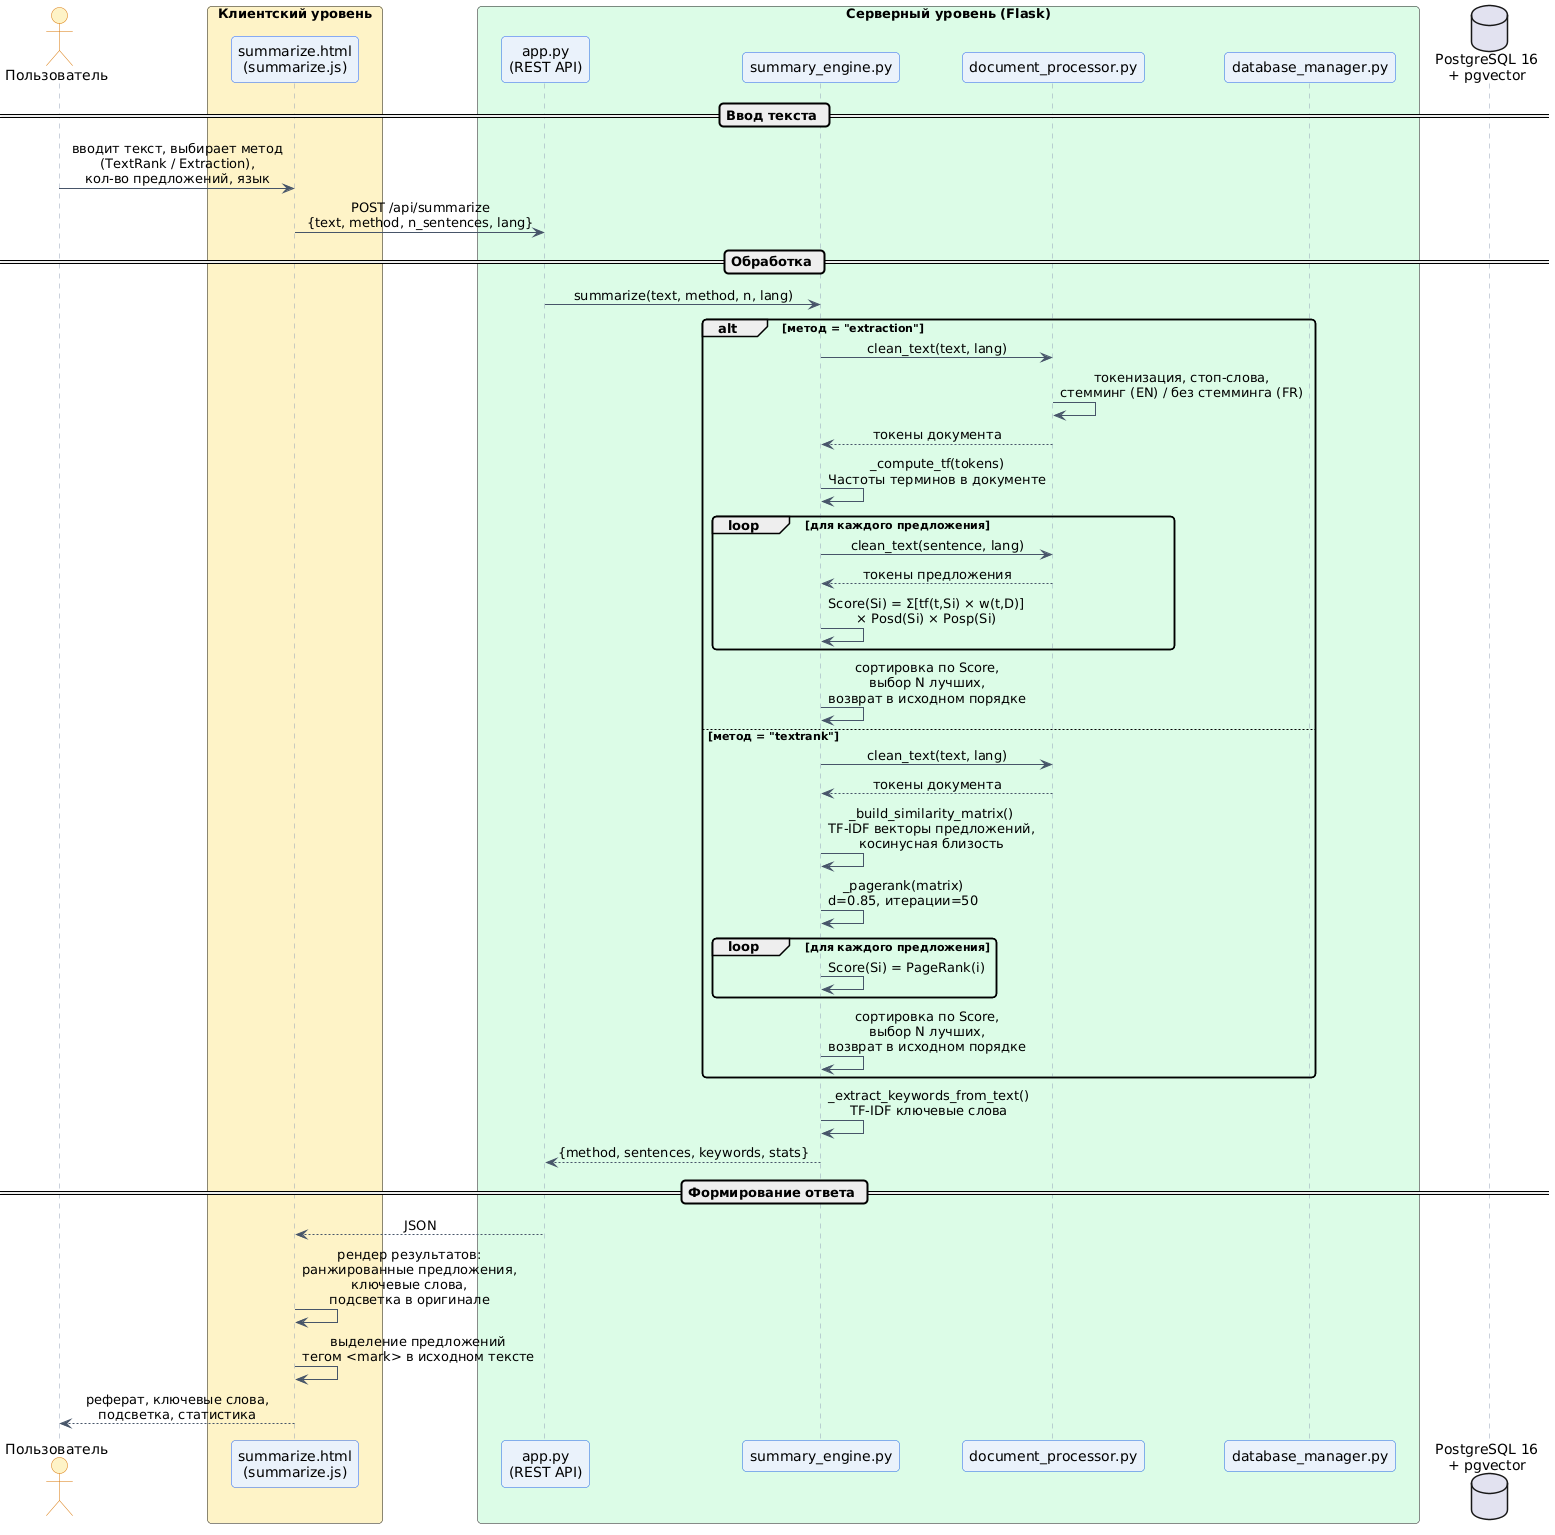
\includegraphics[width=1.0\textwidth]{png/sequence_summarize.png}
	\caption{Диаграмма последовательности реферирования текста.}
	\label{fig:summary_seq}
\end{figure}

\begin{figure}[H]
	\centering
	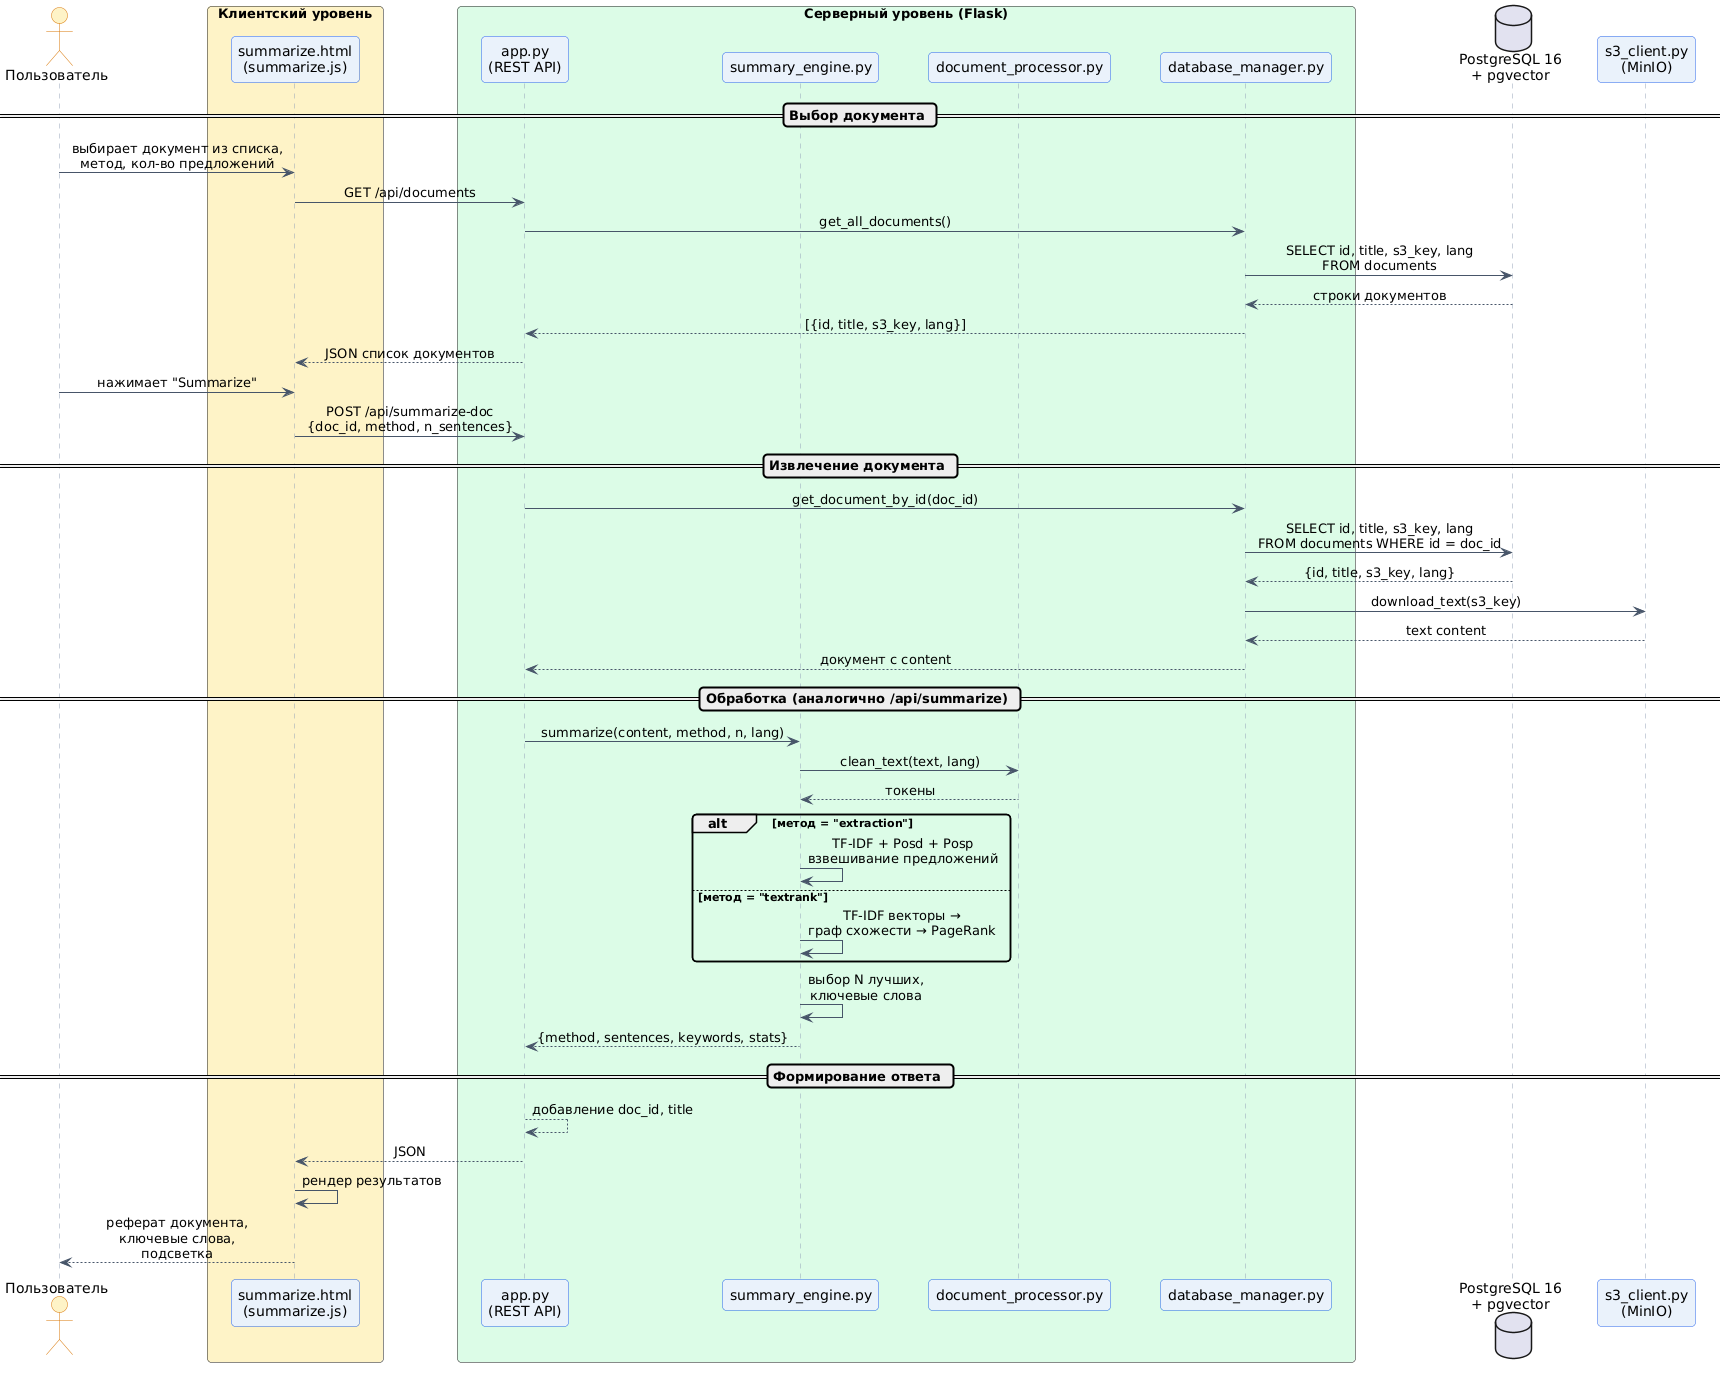
\includegraphics[width=1.0\textwidth]{png/sequence_summarize_doc.png}
	\caption{Диаграмма последовательности реферирования документа из БД.}
	\label{fig:summary_doc_seq}
\end{figure}

\subsection{Метод Sentence Extraction (TF-IDF + позиционные коэффициенты)}

Извлечение предложений "--- извлечительный метод: из исходного текста
отбираются предложения с наибольшим весом и возвращаются в исходном порядке.

\subsubsection{Вычисление веса предложения}

Вес каждого предложения $S_i$ вычисляется произведением трёх компонентов:

\begin{equation}
	\text{Score}(S_i) = \underbrace{\sum_{t \in S_i} \text{tf}(t, S_i) \cdot w(t, D)}_{\text{TF-IDF компонента}} \times \underbrace{\text{Posd}(S_i)}_{\text{позиция в документе}} \times \underbrace{\text{Posp}(S_i)}_{\text{позиция в абзаце}}
	\label{eq:summary_score}
\end{equation}

\textbf{TF-IDF компонента.} Для каждого термина $t$ в предложении $S_i$ вычисляется:

\begin{equation}
	\text{tf}(t, S_i) = \frac{\text{count}(t, S_i)}{|S_i|},
	\qquad
	w(t, D) = \left(0.5 + 0.5 \cdot \frac{\text{tf}(t, D)}{\text{tf}_{\max}(D)}\right) \cdot \text{IDF}(t)
	\label{eq:summary_tf}
\end{equation}

где $\text{tf}(t, S_i)$ "--- частота термина в предложении, $\text{tf}(t, D)$ "--- частота
термина в документе, $\text{tf}_{\max}(D)$ "--- максимальная частота термина в документе,
$\text{IDF}(t) = \log(22 \cdot |DB| / df(t))$ "--- обратная частота документа
(с гладящим множителем 22), $|DB|$ "--- число документов в корпусе,
$df(t)$ "--- число документов, содержащих термин $t$.

\textbf{Позиция в документе (Posd).}

\begin{equation}
	\text{Posd}(S_i) = 1 - \frac{BD(S_i)}{|D|}
	\label{eq:posd}
\end{equation}

где $BD(S_i)$ "--- количество символов до предложения $S_i$ в документе, $|D|$ "--- общее число символов.
Ранние предложения получают больший вес.

\textbf{Позиция в абзаце (Posp).}

\begin{equation}
	\text{Posp}(S_i) = 1 - \frac{BP(S_i)}{|P|}
	\label{eq:posp}
\end{equation}

где $BP(S_i)$ "--- количество символов до предложения $S_i$ в абзаце, $|P|$ "--- длина абзаца.
Первое предложение абзаца получает наибольший вес.

\textbf{Псевдокод метода:}

\begin{lstlisting}[caption={Алгоритм Sentence Extraction.},label={lst:extraction_algo}]
def sentence_extraction(text, n, lang):
    sentences = split_into_sentences(text)
    paragraphs = split_into_paragraphs(text)
    tokens = clean_text(text, lang)
    doc_tf = compute_tf(tokens)
    tf_max = max(doc_tf.values())

    for sent in sentences:
        tokens = clean_text(sent, lang)
        sent_tf = compute_tf(tokens)
        score = sum(sent_tf[t] * (0.5 + 0.5 * doc_tf[t] / tf_max)
                    for t in sent_tf)
        score *= position_in_document(sent, text)
        score *= position_in_paragraph(sent, paragraphs)
        scores.append(score)

    top_n = sorted(scores, key=score, reverse=True)[:n]
    return sorted(top_n, key=position)  # исходный порядок
\end{lstlisting}

\subsection{Метод TextRank}

TextRank "--- графовый метод, аналог PageRank для предложений документа.

\subsubsection{Построение графа}

\begin{enumerate}
	\item Каждое предложение $S_i$ представляется TF-IDF-вектором $\vec{v_i}$.
	\item Матрица схожести $W$: $W_{ij} = \cos(\vec{v_i}, \vec{v_j})$ если $\cos > 0$, иначе $0$.
	\item Строки нормируются: $W_{ij} = W_{ij} / \sum_k W_{ik}$.
\end{enumerate}

\subsubsection{Алгоритм PageRank}

\begin{equation}
	\text{PR}(S_i) = \frac{1 - d}{N} + d \cdot \sum_{S_j \in \text{In}(S_i)} \frac{\text{PR}(S_j)}{|\text{Out}(S_j)|}
	\label{eq:pagerank}
\end{equation}

где $d = 0.85$ "--- коэффициент затухания, $N$ "--- число предложений,
$\text{In}(S_i)$ "--- множество предложений, ссылающихся на $S_i$ (с ненулевой схожестью).

Итерации продолжаются до сходимости ($\epsilon = 10^{-6}$) или максимум 50 итераций.

\textbf{Псевдокод метода:}

\begin{lstlisting}[caption={Алгоритм TextRank.},label={lst:textrank_algo}]
def textrank(text, n, lang):
    sentences = split_into_sentences(text)
    matrix = build_similarity_matrix(sentences, lang)
    scores = pagerank(matrix, d=0.85, iterations=50)

    top_n = sorted(zip(scores, sentences),
                   reverse=True)[:n]
    return sorted(top_n, key=position)  # исходный порядок
\end{lstlisting}

\subsection{Извлечение ключевых слов}

Ключевые слова извлекаются по TF-IDF весу для всего документа:

\begin{equation}
	\text{score}(t) = \text{tf}(t) \cdot \text{idf}(t), \qquad
	\text{tf}(t) = 1 + \log(\text{count}(t))
	\label{eq:kw_score}
\end{equation}

Возвращаются $K$ терминов с наибольшим весом (по умолчанию $K = 8$).

\subsection{Многоязычная поддержка}

Параметр \texttt{lang} определяет режим предобработки:

\begin{table}[H]
	\centering
	\begin{tabular}{|p{3cm}|p{5cm}|p{5cm}|}
		\hline
		\textbf{Параметр} & \textbf{English (\texttt{en})} & \textbf{French (\texttt{fr})} \\
		\hline
		Регистр & нижний & нижний \\
		\hline
		Удаление символов & только \texttt{a--z} & сохранение диакритики \\
		\hline
		Стоп-слова & NLTK \texttt{english} & NLTK \texttt{french} \\
		\hline
		Стемминг & Портер & без стемминга \\
		\hline
	\end{tabular}
	\caption{Режимы предобработки для двух языков.}
	\label{tab:summary_lang}
\end{table}

Язык запроса определяется автоматически при загрузке документа
(классификатор из секции~\ref{sec:langdetect}) и передаётся
в модуль реферирования.

\subsection{Результаты тестирования}

Тестирование проводилось на тестовой коллекции из 12 англоязычных
документов (тематика музыки) и 6 французских документов (медицинские
статьи и критика искусства).

\subsubsection{Сравнение методов}

\begin{table}[H]
	\centering
	\begin{tabular}{|p{4cm}|c|c|c|c|}
		\hline
		\textbf{Метрика} & \textbf{Extraction (EN)} & \textbf{TextRank (EN)} & \textbf{Extraction (FR)} & \textbf{TextRank (FR)} \\
		\hline
		Среднее время (с) & 0,004 & 0,026 & 0,005 & 0,028 \\
		\hline
		Средняя степень сжатия (\%) & 20,4 & 20,4 & 19,8 & 19,8 \\
		\hline
		Кол-во предложений (N) & 10 & 10 & 10 & 10 \\
		\hline
	\end{tabular}
	\caption{Сравнительные метрики методов реферирования.}
	\label{tab:summary_methods}
\end{table}

Метод Sentence Extraction работает быстрее (0,004~с) за счёт отсутствия
построения графа; TextRank (0,026~с) учитывает связи между предложениями,
что потенциально повышает качество на длинных документах.

\subsubsection{Пример реферата}

Для документа \texttt{blues\_music.txt} (27 предложений) метод TextRank
выбрал следующие 5 предложений (N=5):

\begin{enumerate}
	\item The Great Migration of African Americans from the rural South to northern cities in the early to mid-20th century brought blues music to new audiences and led to the development of electric blues.
	\item These guitarists demonstrated that the blues was not just a vocal music but also a powerful instrumental tradition.
	\item Blues music has had a profound influence on the development of jazz, rock and roll, and pop music.
	\item The twelve-bar blues progression and blue notes are fundamental elements of rock music.
	\item The Chicago Blues Festival, the King Biscuit Blues Festival, and the Blues on the Green concert series in Austin, Texas are just a few examples of major blues events.
\end{enumerate}

Ключевые слова: \texttt{blue}, \texttt{king}, \texttt{delta}, \texttt{guitarist},
\texttt{chicago}, \texttt{guitar}, \texttt{south}, \texttt{memphis}.

\subsection{Интерфейс системы}

На странице \texttt{summarize.html} реализован интерфейс:

\begin{itemize}
	\item выбор источника: ввод текста или выбор документа из БД;
	\item переключатель метода: TextRank / Sentence Extraction;
	\item ползунок количества предложений (3--20, по умолчанию 10);
	\item выбор языка (EN / FR);
	\item результат: ранжированные предложения с весами, ключевые слова,
	подсветка предложений в исходном тексте, статистика обработки.
\end{itemize}

\subsection{Выводы по разделу}

Реализована подсистема автоматического реферирования документов с двумя
извлечительными методами: TF-IDF с позиционными коэффициентами и TextRank.
Методы работают с документами на английском и французском языках, переиспользуя
существующую инфраструктуру предобработки. Subsystem интегрирована в
клиент-серверную архитектуру ИПС и доступна через REST API и веб-интерфейс.
